% !TEX root=../mt-motion-analysis.tex
\chapter{Introduction}

skriv om risker med bias fr dataset osv...

\section{Medical background}
skriv om acl och varf;r detta arbete beh;vs
related work, se ref i mendeley osv
\subsection{POEs}
...

\section{Machine learning} \label{sec:ML}
skriv om att ml blivit s[ stort sen alexnet och gpu osv

The emergence of computing power discussed in Section \ref{sec:ML} allowing deeper networks shown by AlexNet \cite{Krizhevsky2012}

\section{Pose estimation} \label{sec:pose_estimation}
Human pose estimation is a well explored problem which, like many other computer vision tasks has developed rapidly in the recent years. The reasons behind this progress can mainly be explained by two factors. Firstly the emergence of computing power discussed in Section \ref{sec:ML}, allowing more powerful deep learning models. Secondly several datasets with images labeled with human body joints has been made available \cite{Chen2020}. These datasets not only provide data, but also introduces competition in the research community making it possible to compare the results of different approaches.

\subsection{Datasets}
Some of the widely used datasets today are Max Planck Institute for Informatics (\textbf{MPII}) \cite{Andriluka2014}, Microsoft Common Objects in Context (\textbf{COCO}) \cite{Lin2014}, AI Challenger Human Keypoint Detection (\textbf{AIC-HKD}) \cite{Wu2017}, and COCO-wholebody \cite{Jin2020}.% The two COCO datasets will now be described in more detail.

The COCO dataset consists of 328k images containing 91 different object types. The images come from Google, Bing, and Flickr image search and are mainly hand annotated through Amazon  Mechanical Turk. The interesting part of the dataset for this work is the one with human poses. In total there are 250k instances of people labeled with joint locations \cite{Lin2014}. The joints, 13 per person, in the dataset can be seen in Figure \ref{fig:coco}. Along with the datasets containing body keypoints mentioned above there are also datasets with dense keypoints for specific bodyparts, e.g. OneHand10k \cite{Wang2019}. COCO-wholebody is an attempt to combine these two types of datasets by extending COCO with dense keypoints at hands, feet, and faces. The resulting 133 joints can be seen in Figure \ref{fig:coco-wholebody}.

\begin{figure}
 \centering
 \begin{subfigure}[t]{0.4\textwidth}
  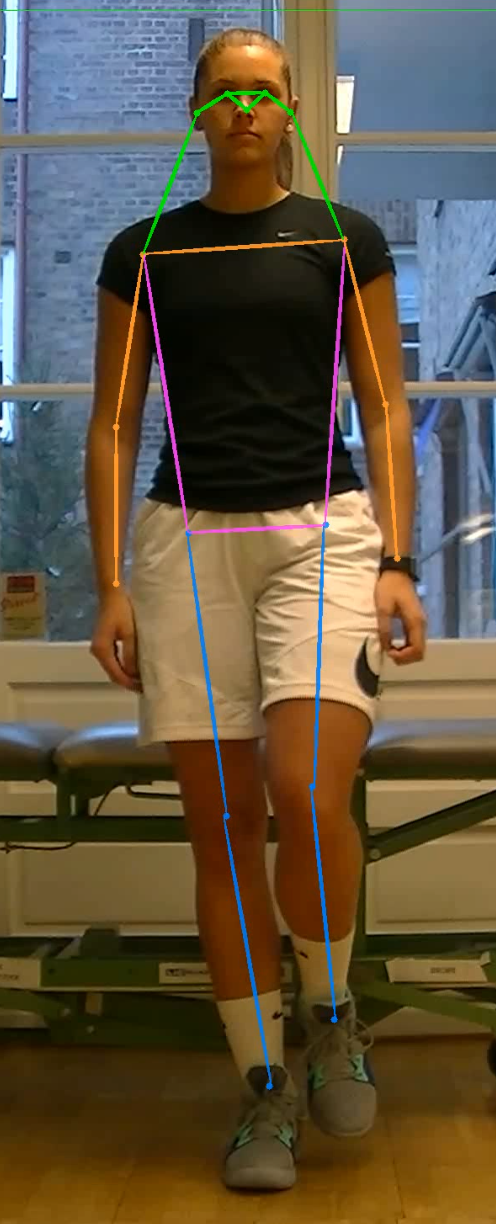
\includegraphics[width=\textwidth]{files/figs/coco.png}
  \caption{Regular COCO.}
  \label{fig:coco}
 \end{subfigure}
 ~
 \begin{subfigure}[t]{0.4\textwidth}
  \includegraphics[width=\textwidth]{files/figs/coco-whole.png}
  \caption{COCO-wholebody.}
  \label{fig:coco-wholebody}
 \end{subfigure}
 \caption{Keypoints for the two COCO datasets.}
\end{figure}
% The two COCO datasets will now be described in more detail. These are extensi
% The two COCO datasets are

% \subsubsection{COCO}





\section{Time series classification}
\cite{IsmailFawaz2019}

% \subsubsection{??}
